%%This is the evaluation part, int includes the following parts.
% <1> Evaluation Metrics, explain the measurements chosen for this experiments
% <2> Test Platform in KNIME, introduced before so we don't really need to repeat it here
% Firstly, we validate our methods and make sure it works for the properties.. Then using the whole data to test the weights tend and also, if it handled the real life data. 
% <3.1> validation part to check the methods work for those situations, but not necessary;; Then big data test to show property to handle those situations. 
% <3> Test Cases Design, the parameters we want to compare, the cases
%   ==> synthetic data
%   ==> Real life data
%   ++ Data to test the property
In this chapter, we evaluate the proposed repair techniques based on the quality of repaired model. At first, we define the evaluation criteria. Next, we briefly introduce the test platforms KNIME and relevant ProM plugins tools. Then, we conduct two kinds of tests. One is based one the demo example proposed in the introduction part, and the other is on the real life data. 
\section{Evaluation Criteria}
% First talk about our data and our model, then choose the confusion matrix as one measurements. But we should review the traditional measuremtns on process mining before introducing the confusion matrix. but we should also focus on the accuracy part and f-score.
We evaluate the repair techniques based on the quality of repaired models with respect to the given event logs. In process mining, there are four quality dimensions generally used to compare the process models with event logs. 
\begin{itemize}
	\item \emph{Fitness.} It quantifies the extent how well the model reproduces traces in the event log which is used to build the model.   
	\item \emph{Precision.} It quantifies the extent how the discovered model limits the completely unrelated behavior that doesn't show in the event log. 
	\item \emph{Generalization.} It addresses the over-fitting problem when a model strictly matches to only seen behavior but is unable to generalize the example behavior seen in the event log. 
	\item \emph{Simplicity.} This dimension captures the model complexity. According to Occam's razor principle, the model should be as simple as possible.
\end{itemize}
% How to come to confusion matrix?? 
The four traditional quality criteria are proposed in the environment where only positive instances are available. Therefore, when it comes to the model performance, where negative instances are also possible, the measurement metrics need to be adjusted. 

With labeled traces in the event log, the repaired model can be seen as a binary prediction model where the positive instances are supported while the negative ones are rejected. Consequently, the model evaluation becomes a classifier evaluation and confusion matrix is applied in our experiments.

% Describe its features and some derived measurements. 
Confusion matrix has a long history to evaluate the performance of a  classification model. A confusion matrix is a table with columns to describe the prediction model and rows for actual classification on data.  As seen as a binary classifier, the repaired model produces four outcomes according to confusion matrix -- true positive, true negative, false positive and false negative, which is shown in the Table \ref{tab:cm}.
\begin{itemize}
	\item True Positive(TP): The execution allowed by the process model has a positive performance outcome.
	\item False Positive(FP): The execution allowed by the process model has a negative performance outcome.
	\item True Negative(TN): The negative instance is blocked by the process model.
	\item False Negative(FN):The negative instance is enabled by the process model.
\end{itemize} 
% confusion matrix
\begin{table}[]
	\caption{Confusion Matrix}
	\label{tab:cm}
	\begin{tabular}{ll|c|c|}
		\cline{3-4}
		&                   & \multicolumn{2}{c|}{repaired model}                                               \\ \cline{2-4} 
		\multicolumn{1}{l|}{}                                                                         &                   & \multicolumn{1}{l|}{allowed behavior} & \multicolumn{1}{l|}{not allowed behavior} \\ \hline
		\multicolumn{1}{|l|}{\multirow{2}{*}{\begin{tabular}[c]{@{}l@{}}actual \\ data\end{tabular}}} & positive instance & TP                                    & FN                                        \\ \cline{2-4} 
		\multicolumn{1}{|l|}{}                                                                        & negative instance & FP                                    & TN                                        \\ \hline
	\end{tabular}
\end{table}
Various measurements can be derived from confusion matrix. According to our application, the following criteria are chosen. Generally, there is a trade-off between the quality criteria. So the measurements below are only used to evaluate specific aspects of repair techniques.
\begin{itemize}
	\item Recall. It represents the true positive rate and is calculated as the number of correct positive predictions divided by the total number of positives.
	\[Recall = \frac{TP}{TP + FN}\]
	\item Precision. It describes the ability of the repaired model to produce positive instances.
	\[Precision = \frac{TP}{TP + FP }\]
	%\item specificity. In opposite with recall, it measures the true negative rate.
	%\[Specificity = \frac{TN}{TN + FP}\]
	\item Accuracy. It is the proportion of true result among the total number. It  measures in our case how well a model correctly allows the positive instances or disallows the negative instances.
	\[Accuracy = \frac{TP+TN}{TP+TN+FP+FN}\]
	\item F-score is is the harmonic mean of precision and recall.
	\[F_1 = \frac{2*Recall*Precision}{Precision + Recall}\]
\end{itemize}

\section{Experiment Platforms}
KNIME, as a scientific workflow analytic platform, supports automation of test workflow, which helps us repeat experiments efficiently. Yet, the integration of traditional process mining plugins into KNIME is out of our capability due to the time limit. Therefore, partial experiments with current repair techniques are still conducted in ProM. 
\subsection{KNIME}
% this section describes how KNIME supports automatic test, FlowVariable and optimization parts of it.
KNIME supports automation of test workflow mainly through the following mechanisms. 
\begin{itemize}
	\item Loop Control Structure. KNIME provides a bunch of control nodes which support re-executing workflow parts.  Two nodes \emph{Loop Start} and \emph{Loop End} explicitly express the beginning and end of a loop structure, where the workflow between those two node is the loop body and is executed recursively in a fixed number, or until certain conditions are met. In our test, we repeat our repair techniques for different parameter settings by applying loop structure into KNIME workflow.
	\item Flow Variables. Flow Variables are used inside a KNIME workflow to parameterize node settings dynamically. When it combines with loop control structure, tests with different settings is able to conduct automatically.
\end{itemize}
Furthermore, there are nodes provided by KNIME to optimize the value of some parameters with respect to a cost function. As long as the cost function is provided, KNIME is able to automatically optimize the corresponding parameters. 

\subsection{ Experiments with ProM Plugins}
Due to the frequent errors on the corresponding plugin, we exclude the tests on repair techniques in \cite{dees2017enhancing} and conduct experiments with the following types. 
\begin{itemize}
	\item \textbf{Type 1} \textbf{Inductive Miner} only on the positive event log to discover a model. The default setting with infrequent variant and noise threshold as 20 is chosen. Later, the mined model is checked on the labeled event with positive and negative instances. This method is abbreviated as IM.
	\item \textbf{Type 2} \textbf{Repair Model} from \cite{fahland2015model} is applied on the positive event log to discover a model. The default setting is chosen. Later, the mined model is checked on the labeled event with positive and negative instances. This method is abbreviated as Fahland, named after the name of main author.
	\item \textbf{Type 3} \textbf{Dfg-Repair from our thesis} is applied on the labeled event log with positive and negative instances. Default setting  for the control parameters is 1.0 while the parameters to generate Petri nets from directly-follows graph are set as the same as experiment Type 1.  Later, the repaired model is evaluated on the labeled data. 
\end{itemize}

\section{Experiment Results}
We conduct our experiments into two main parts. One is to verify if our method overcomes the limits of current repair algorithms. This experiment is based on the synthetic data and models from Introduction chapter. The other experiment is based on real life data, in order to test the feasibility of our repair techniques.
%For convenience,we refer the repair methods in \cite{fahland2015model} by the main auther's name Fahland, and the repair techniques in \cite{dees2017enhancing} as Dees. The Inductive Miner is abbreviated as IM. Our method which built on directly-follows graph is denoted as Dfg-repair. 
 
\subsection{Test on Demo Example}
In this part, experiments are performed on the motivating examples which are listed in Introduction. Thereby, we are able to answer whether our repair method overcomes shortcomings of current techniques which are shown in the introduction chapter. 
\subsubsection{Answer to Situation 1}
\emph{Situation 1} shows the drawbacks of current repair methods \cite{fahland2015model, dees2017enhancing} that unexpected behaviors are introduced into model by adding subprocess in the form of loops. Moreover, rediscover strategy with IM doesn't take the original model into account and generates a new model that deviates from the original model. 


Given the process model $M_0$ and the event log $L_1$, additional activities \textbf{x1,x2} in $L_1$ lead to good performance and need to be added into the model $M_0$. Applying proposed repair techniques dfg-repair, we obtain the  repaired model listed in Figure \ref{fig:demo_dfg_s1}. The parameters for our method are set in the following : weight for the existing model is 0.45, weight for positive examples is 1.0, the Inductive Miner for Infrequent is chosen and has a noise with 20, which is the same setting as the rediscovery method by Inductive Miner in Introduction. 

As seen in Figure \ref{fig:demo_dfg_s1}, the subprocesses for \textbf{x1,x2} are added in a sequence with others. In this way, $M_{1.3}$ is able to reflect the deviations in positive instances while keeping similar to the reference model $M_0$. Compared to techniques in \cite{fahland2015model}, it increases the precision without loops.
% we should give our confusion matrix result
\begin{figure}[htp]
	\centering
	\begin{subfigure}[b]{0.31\textwidth}
		\centering
		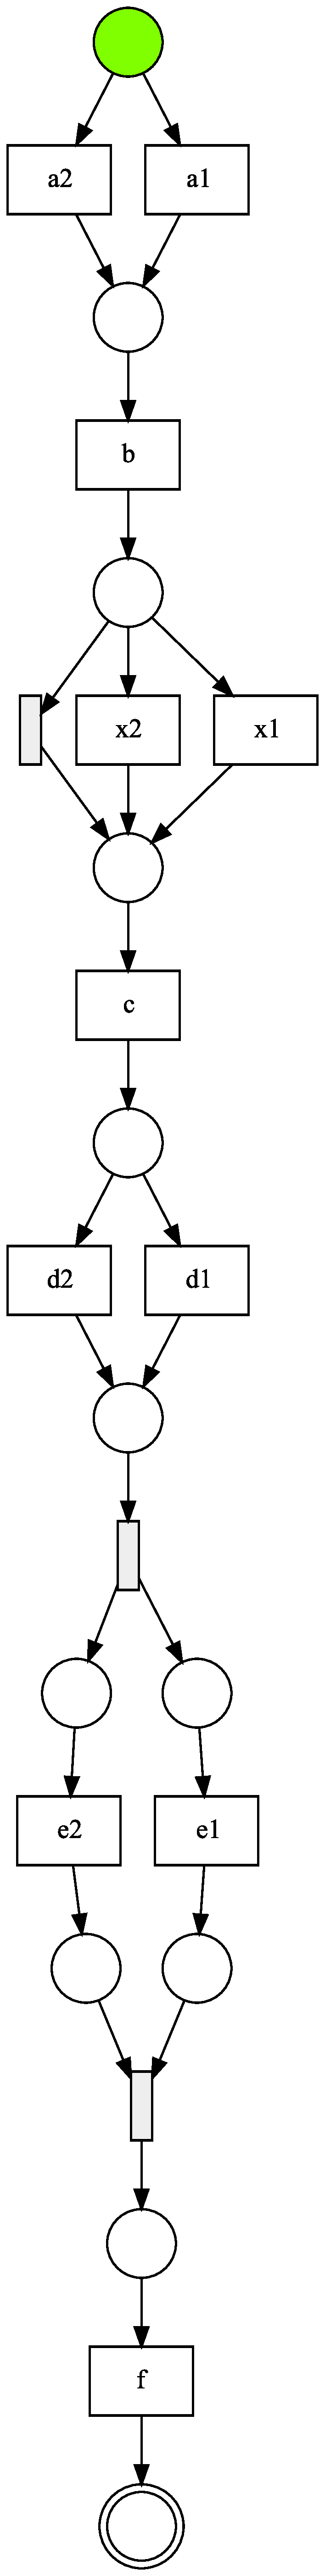
\includegraphics[width=0.75\linewidth, height=0.8\textheight]{figures/evaluation/PN-result-demo-s1-dfg.pdf}
		\caption{$M_{1.3}$ for situation 1}
		\label{fig:demo_dfg_s1}
	\end{subfigure}%
\quad
	\begin{subfigure}[b]{0.31\textwidth}
		\centering
		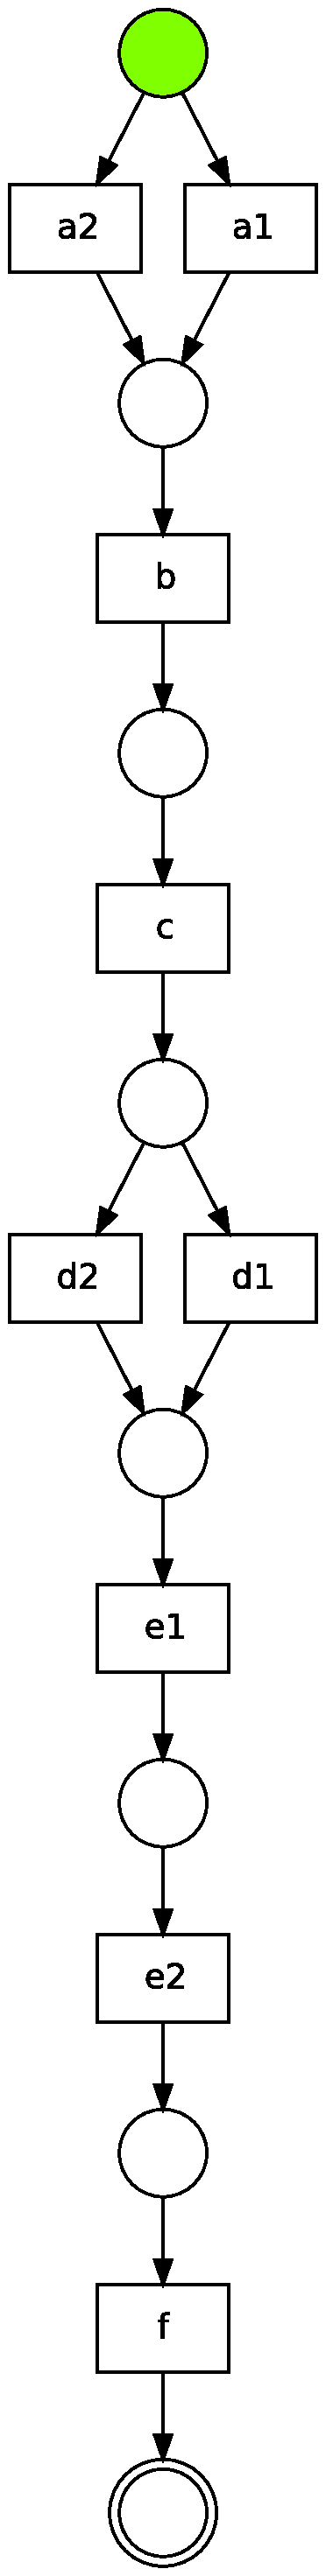
\includegraphics[ width=0.75\linewidth, height=0.8\textheight]{figures/evaluation/PN-result-demo-s2-dfg.pdf}
		\caption{$M_{2.3}$ for situation 2}
		\label{fig:demo_dfg_s2}
	\end{subfigure}
 \quad
\begin{subfigure}[b]{0.32\textwidth}
	\centering
	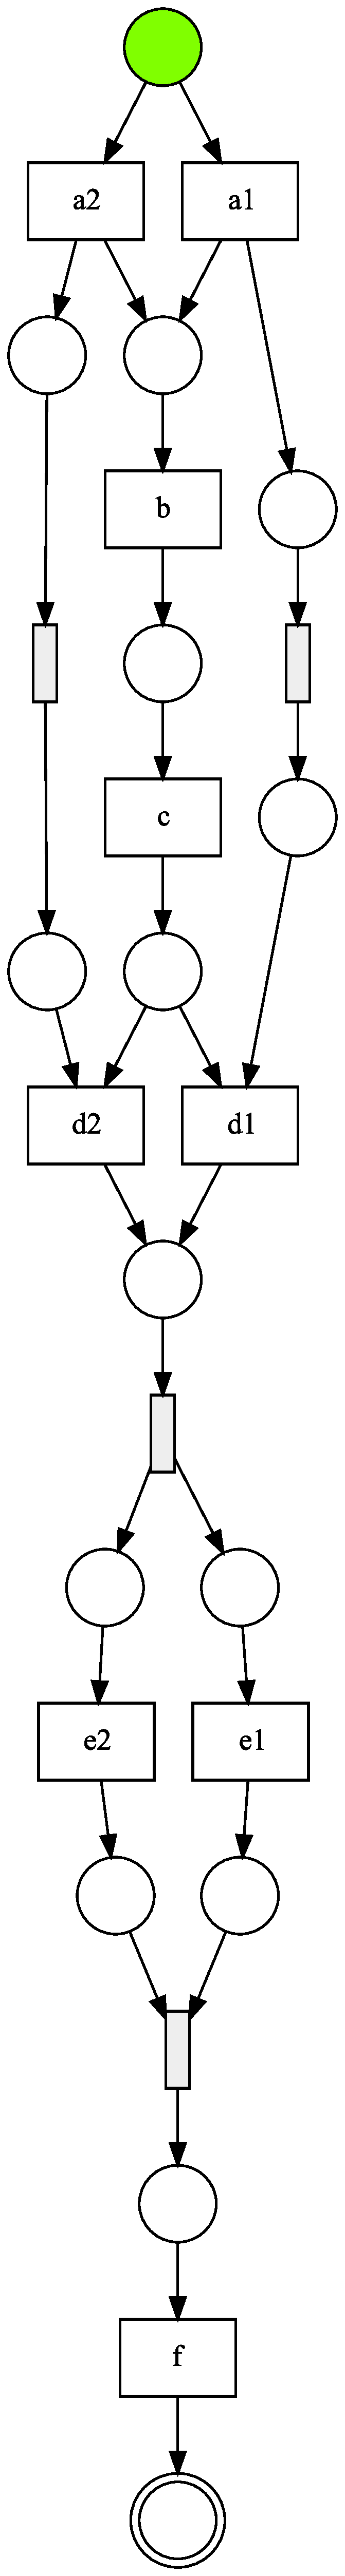
\includegraphics[ width=0.75\linewidth, height=0.8\textheight]{figures/evaluation/PN-result-demo-s3-dfg.pdf}
	\caption{ $M_{3.3}$ for situation 3}
	\label{fig:demo_dfg_s3}
\end{subfigure}
	\caption{repaired models with our techniques for situation 1,2 and 3 in Introduction part. The green place is the initial marking of the Petri net and the doubled place is the final marking.}
	\label{fig:demo_dfg}
\end{figure}
\subsubsection{Answer to Situation 2}
Situation 2 describes the inability of current repair methods that fitting traces with negative performance outcomes cannot be used to repair a model. 
% some explaination about the situation.
The execution order of \textbf{e1, e2} affects the performance outcomes and \textbf{e1} is expected to position before \textbf{e2}. Without negative information, the repaired models have the same structure as the reference ones, because the execution of \textbf{e2} before \textbf{e1} brings also the positive outcomes. 

If we apply our repair methods on the model $M_0$ and event log $L_2$, with 1.0 for all control weights, and the same Inductive Miner-Infrequent with noise 20, the repaired model $M_{2.3}$ is obtained. In $M_{2.3}$, \textbf{e1} is executed before \textbf{e2}. It shows that our method is able to incorporate the negative information and balance the forces from the existing model, positive and negative instances. 

\subsubsection{Answer to Situation 3}
% Conclusion part
Situation 3 concerns the long-term dependency in Petri nets, which is not handled in current repair and rediscovery techniques. As observed in event log, there exists the long-term dependency set, $LT=\{ a1\rightsquigarrow d1, a2\rightsquigarrow d2\}$.  With adding long-term dependency as expected in Figure \ref{fig:demo_s3_expected}, precision and accuracy increase, since the model limits activity selection and blocks the negative behavior due to free execution of xor branches. Yet none of the current repair  and rediscovery techniques are able to detect and add long-term dependencies in the Petri net. 

In our repair techniques, the long-term dependency is taken into account with negative information. With inputs of the Petri net $M_0$ and event log $L_3$, our methods produces the repaired model $M_{3.3}$ with long-term dependency. Two silent transitions that are used to explicitly represent the long-term dependencies can be deleted with post procedure to reduce the redundant silent transitions and places. After reduction, our repaired model is simplified as the model $M_{3}$. 
\subsubsection{Comparison with Confusion Matrix}
In this section, we list the evaluation results of the repaired models based on confusion matrix. In Table \ref{tab:demo-result}, for Situation 1 with only positive instances, the repair techniques give the same confusion matrix result. However,  $M_{1.2}$  with loops implicates a lower precision. In Situation 2, with current techniques or rediscovery methods in IM, the model stays the same as the reference  model $M_0$. Since no negative instance is rejected, the recall is 1 but precision is below 0.6.  In comparison, dfg-repair uses the negative instances and adjusts the model correspondingly. Therefore, the repaired model $M_{2.3}$ has higher precision, accuracy and F1 score. In Situation 3 with long-term dependency, our method succeeds to detect and add the  long-term dependency in the model. In this way, no false positive or false negative instances are in the confusion matrix, and the repaired model holds the highest values for all listed measurements.
\begin{table}[h]
	\centering
	\caption{Test Result on BPI15-M1 data}
	\label{tab:demo-result}
	\resizebox{\textwidth}{!}{
		\begin{tabular}{lll|llllllll|}
			\hline
			\multirow{2}{*}{\thead{Situation}} & \multirow{2}{*}{\thead{method} }                &    \multirow{2}{*}{\thead{Generated \\ model}}       & \multicolumn{8}{l|}{ \thead{confusion matrix metrics}}                                \\
			\cline{4-11}
			&  &     &
			\thead{TP}  & \thead{FP} & \thead{TN}  & \thead{FN}  & \thead{recall} & \thead{precision} & \thead{accuracy} & \thead{F1}             \\
			\hline
			S1      & IM              & $M_{1.1}$ & 50 & 50 & 0 & 0 & 1   & 0.5     & 0.5     & 0.667               \\
			S1     & Fahland              & $M_{1.2}$   & 50   & 50  &0     &0     & 1   & 0.5     & 0.5     & 0.667               \\
			
			S1      & Dfg-repair              &    $M_{1.3}$    &  50   &  50  &  0  &    0 &  1   & 0.5     & 0.5     & 0.667               \\
			
			\hline
			S2      & IM/Fahland              & $M_0$   & 60    & 45   &  0  & 0    &  1     &    0.571       & 0.571         &  0.727   \\
			
			S2      & Dfg-repair              & $M_{2.3}$      & 50    &   5 &   40  & 10    &  0.833      &   0.909        &  0.857         &  0.870      \\
			
			\hline
			S3     & IM/Fahland             & $M_{0}$   & 100    & 100   &  0   &  0   &  1.0      &   0.5        &   0.5       &  0.667    \\
			
			S3      & Dfg-repair             & $M_{3.3}$       &  100   &   0 &  100   &  0   &  1      &   1        &  1        &   1     \\
			\hline         
	\end{tabular}}
\end{table}

In conclusion, our proposed method is able to overcome shortcomings of current techniques mentioned in the Introduction. It avoids the loops in model by repairing the model with additional activities, incorporates the negative information in the data to adjust the model, also detect and add the long-term dependency into model. In this way, the repaired model has better  recall, and accuracy.

\subsection{Test on Real Life Data}
% here we will list all the data here but before describe the test data
We choose publicly available event logs from BPI challenge 2015 and build a data set from them to test the feasibility of proposed repair techniques.
\subsubsection{Data Description}
The data set for BPI Challenge 2015 contain 5 event logs which are provided by five Dutch municipalities respectively. Those event logs describe the building permit application around four years. We choose it as our user cases due to the following reasons.
\begin{itemize}
	\item The event logs hold attributes as potential KPIs to classify traces. Attribute \textbf{SUMleges} which records the cost of the application is a candidate to label traces as positive or negative if its value  is over the threshold. What's more, we can take the throughput time of the application as another potential KPI. \\
	In a word, this data set provides us information to reasonably label traces.
	\item The five event logs describe an identical process, but includes deviations caused by the different procedures, regulations in those municipalities. Also, the underlying processes have changes over four years.\\
	So, this data set gives us a basic process but also allows deviations of the actual event logs and predefined process, which builds the environment for repair techniques.
\end{itemize}
We conduct our experiments on those event logs. However, due to the time limits, we only managed to get the result on experiments with the event log \textbf{BPIC15\_1.xes.xml}. This event log includes 1199 cases and 52217 events in 398 classes. We preprocess the event log and get a proper subset of data as our user case.  
\begin{table}[h]	
	\caption{Test event log from real life data BPI15-1}
	\label{tab:event-log}
	\begin{tabular}{|l|l|l|l|l|}
		\hline
		Data ID & Data Description                                & Traces Num & Events Num & Event Classes \\ \hline
		D1      & \makecell{Heuristic filter  \\ with 40 }                     & 495        & 9565       & 20             \\ \hline
		D2      & \makecell{Apply heuristic filter \\ on D1 with 60      }     & 378        & 4566       & 12            \\ \hline
		D3.1    & \makecell{classify on SumLedges;  \\ values below 0.7 as positive} & 349        & 6744       & 20             \\ \hline
		D3.2    & \makecell{classify on SumLedges;  \\ values above 0.7 as negative }& 146        & 2811       & 20             \\  \hline
		D3.3    & union of D3.1 and D3.2                             & 495        & 9596       & 20             \\ \hline
		D4.1    & \makecell{ classify on throughput time;  \\ values below 0.7 as positive} & 349        & 6744       & 20             \\ \hline
		D4.2    & \makecell{classify on throughput time;  \\ values above 0.7 as negative} & 146        & 2811       & 20            \\ \hline
		D4.3    & union of D4.1 and D4.2                             & 495        & 9596       & 20           \\ \hline
	\end{tabular}
\end{table}

We filter the raw event log by \textbf{\emph{Filter Log By Simple Heuristic}} in ProM with the following setting. 40 for the start, end  activities and the events between them, at end. We get the event log $D1$. After this, we calculate the throughput time for each trace and add it as a trace attribute \textbf{throughput time}. 
Then we classify traces according to  \textbf{SUMleges} and  \textbf{throughput time} separately. When our performance goal is to reduce the cost of application, if \textbf{SUMleges} of one trace is over 0.7 of the whole traces, this trace is treated as negative, else as positive. The similar strategy is applied on the attribute \textbf{throughput time}. A trace with \textbf{throughput time} higher than 0.7 of all traces is considered as a negative instance. Following this preprocess, we have event logs in Table \ref{tab:event-log} available for our tests. 


\begin{table}[htp]
	\caption{Generated reference models for test}
	\label{tab:ref-models}
	\resizebox{\textwidth}{!}{
	\begin{tabular}{|llll|lllllllll|}
		\hline
		\multirow{2}{*}{\thead{Model\\ ID}} & \multirow{2}{*}{\thead{Used \\Data}} & \multirow{2}{*}{\thead{Setting}}  &  
		\multirow{2}{*}{\thead{Event\\Class}} & \multicolumn{8}{c|}{\thead{CM Evaluation}}                     \\ 
		\cline{5-13}
		&                                                                           &                                                                             &                                                                            &Data & TP & FP & TN & FN & recall & precision & accuracy & F1 \\ \hline
		M1                                                                      & D1                                                                        & \makecell[l]{IM-infrequent: \\ Noise Setting: 20} & 20                                                                         & D3.3 & 112   & 40   & 106   & 237   & 0.321       &0.737           &   0.440       &   0.447 \\
		
		&                                                                      & &                                                                          & D4.3 & 131   &  21  &  128  & 215   & 0.379       & 0.862           & 0.523          & 0.526    \\
		
		\hline
		M2                                                                      & D1                                                                        & \makecell[l]{IM-infrequent: \\ Noise Setting: 50} & 20                                                                         & D3.3 & 106   & 39   &  107  & 243    & 0.304        &  0.731         &0.430          &0.429    \\
		
		&                                                                      & &                                                                          & D4.3 & 125   &   20 & 129   &221    &    0.361    & 0.862           & 0.513          &0.509    \\
		\hline
		
		M3                                                                      & D2                                                                        & \makecell[l]{IM-infrequent: \\ Noise Setting: 20} & 12                                                                         &D3.3 &  0  & 0   & 146   & 349   & 0       &NaN           &    0.295      & 0   \\
		
		&                                                                      & &                                                                          & D4.3 &  0  & 0   & 149   & 346   & 0       & NaN           &  0.301        &0    \\
		\hline 
		
		M4                                                                      & D2                                                                        & \makecell[l]{IM-infrequent: \\ Noise Setting: 50} & 12                                                                         &D3.3 &  0  &  0  &  146  & 349   & 0       & NaN           &     0.295     & 0\\   
		&                                                                      & &                                                                          & D4.3 &  0  & 0   & 149   & 346   & 0       & NaN           &  0.301        &0    \\
		
		\hline
	\end{tabular}
 }
\end{table}
Based on the filtered data, we derive corresponding Petri nets as reference process models. The Table \ref{tab:ref-models} lists the models with different setting. \textbf{IM-infrequent} is one variant of Inductive Miner working on event logs with infrequent traces. \textbf{Noise} is set as the threshold to filter out infrequent traces. After mining a reference model, we compare them with  corresponding event logs to get the basis lines for later evaluation.
% should we explain the data and the model, they are different with old files!!
% Please add the following required packages to your document preamble:
% \usepackage{multirow}

As seen in table above, the reference models don't apply well to the corresponding event logs. So changes on the models are in demand, to reflect better the reality and also to enforce the positive instances and avoid negative instances. 
\subsubsection{Test Result}
% we don't need to transfer page to landscape view, because we have many rows too.
Three types of repair techniques which are called \textbf{IM}, \textbf{Fahland} and \textbf{Dfg-repair} are applied on preprocessed event log set in Table \ref{tab:event-log} and models from Table \ref{tab:ref-models}. The experiment result is listed in the Table \ref{tab:rl-result}. For better understanding, we give the details of one experiment set which is conducted with the reference model M3 and event log D3.1 and D3.3.  

Figure \ref{fig:rl_ref} displays the reference model M3, which has 0 TP and 0 FP compared to D3.3. It implies that M3 leads to no positive performance outcomes. Firstly, Inductive Miner for infrequent traces with noise threshold 0.2 is used on the positive event log D3.1 to rediscover a model. The generated model is shown in Figure \ref{fig:rl_IM}, which has changed a lot compared to the original model M3 as shown in the Figure \ref{fig:rl_ref}. After getting the generated model, we compare it with labeled event log D3.3 and compute the confusion matrix criteria. As shown in Table \ref{tab:rl-result}, the repaired model tend to have high FN and low FP, because the 

 
Since IM doesn't take the reference models into account, it always output the same model based on the event log. 

After applying the Fahland's repair techniques from \cite{fahland2015model}, the reference model M3 is repaired as in Figure \ref{fig:rl_fahland}. With duplicated transitions, loops and silent transitions for adding subprocesses, it is more complicated than the reference model M3. When evaluating the repaired model with confusion matrix, we get 349 TP, 145 FP, 1 TN, and 0 FN, which leads to high recall. However, it needs to notice that the principle of Fahland repair techniques is to add subprocesses for deviations in the model. Without consideration of eliminating negative behavior, the repaired model is likely to damage the model precision and accuracy.

Dfg-repair techniques are firstly applied with the default setting, 1 for all control parameters. It results in a model with 0 TP, 0 FP, 146 TN, and 349 FN,  which contrasts the result by Fahland repair techniques. This is probable because the forces from the existing model and negative instances exceed the positive force, and blocks  behavior with positive outcomes. 

As a comparison, we change the control parameter setting to 0.5 for the existing model, 1 for the positive instances, 0.5 for the negative instances. After repeating the experiment, the confusion matrix changes to 131 TP, 63 FP, 83 TN, and 217 FN, while recall increases from 0 to 0.378, accuracy from 0.294 to 0.428, and F1 from 0 to 0.485. Apparently, the quality is improved due the the new setting. The possible reason is that three forces are balanced more properly for the repaired model.

% here to fix the evaluation from last step!! Better to give a good result on it!! Put it aheda before the whole result, and then organize it later.
\begin{figure}[htp]
	\centering
	\begin{subfigure}[b]{0.45\textwidth}
		\centering
		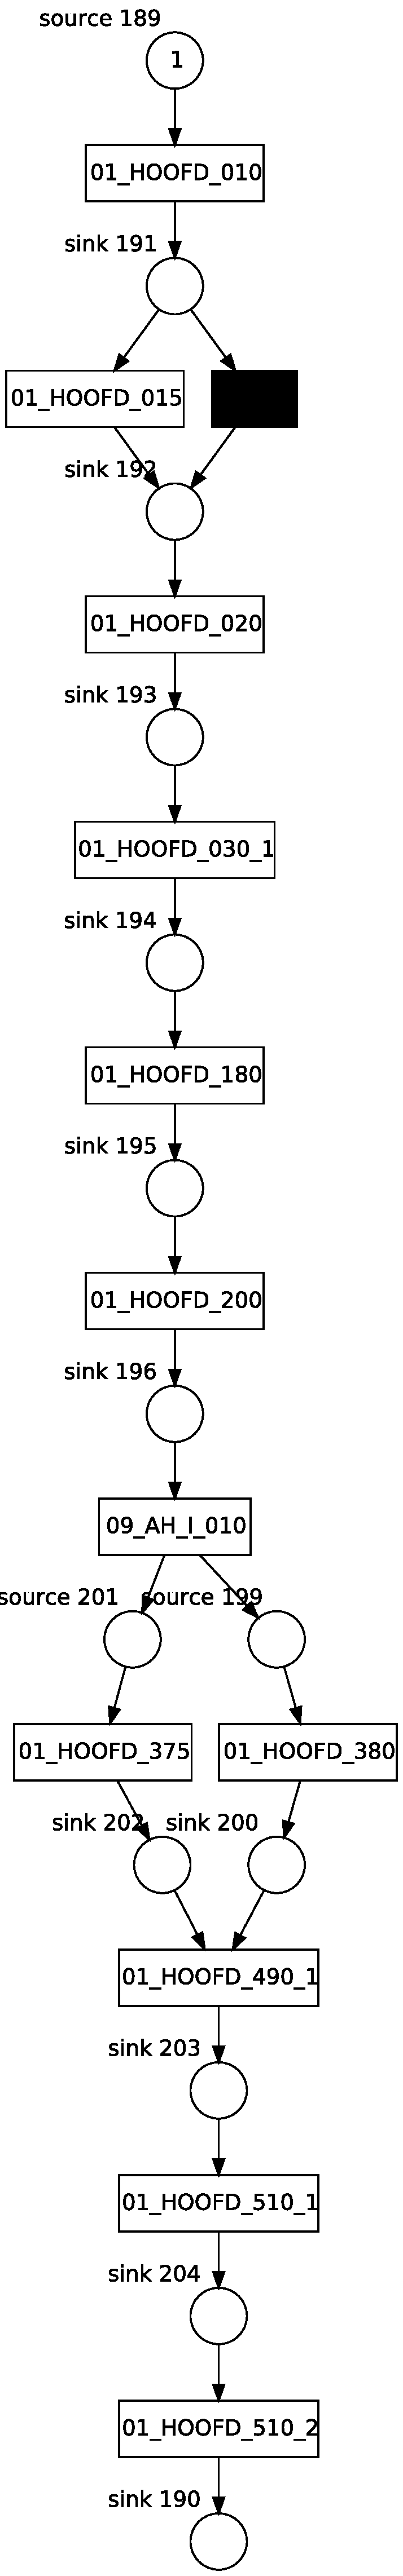
\includegraphics[width=0.7\textwidth, height=0.9\textheight]{figures/evaluation/BPI_1_40_M3_figure.pdf}
		\caption{reference model M3}
		\label{fig:rl_ref}
	\end{subfigure}%
\quad
\begin{subfigure}[b]{0.45\textwidth}
	\centering
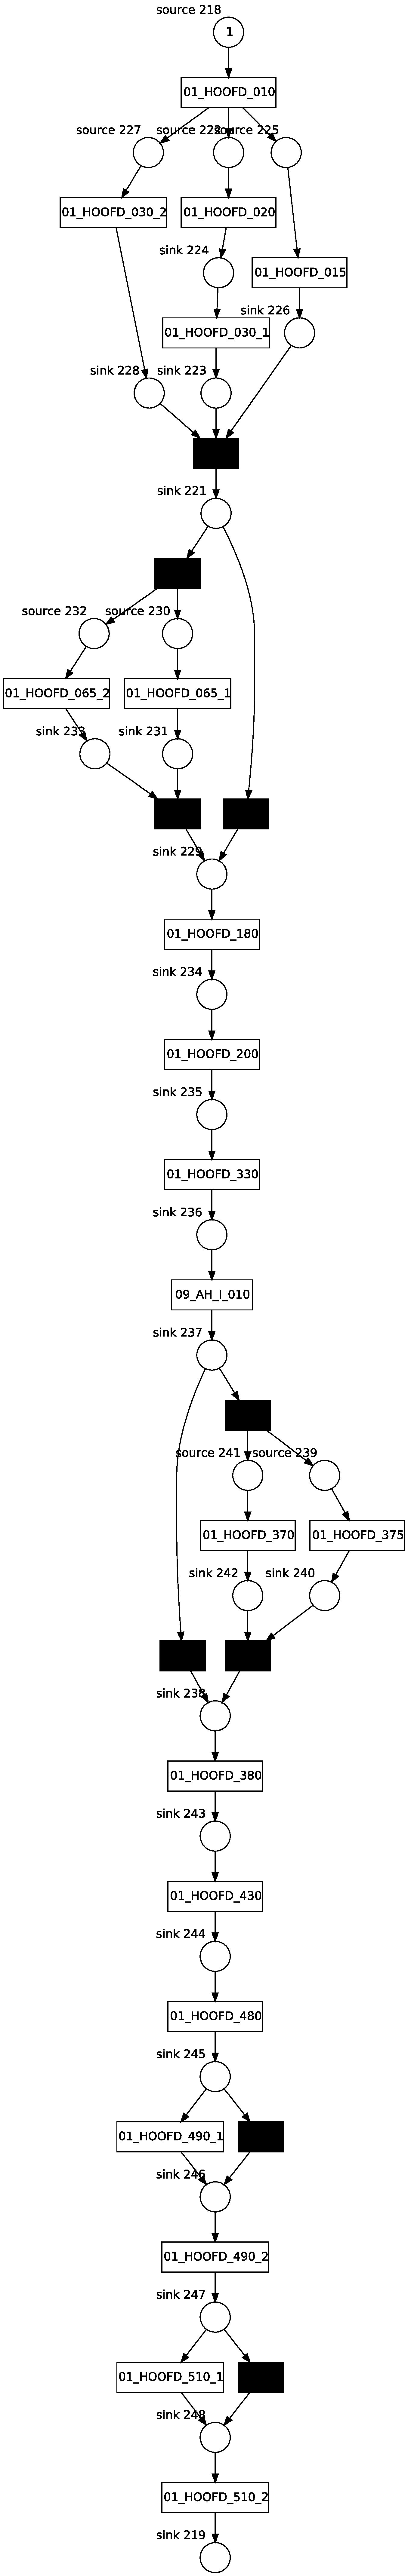
\includegraphics[width=1.0\textwidth, height=0.9\textheight]{figures/evaluation/PN-result-D4-1-IM20-pos.pdf}
\caption{repaired model with IM}
\label{fig:rl_IM}
\end{subfigure}%
\caption{The left model is the reference model M3. The rediscovery algorithm IM generates a new model based on the positive instances which is shown in the right side.}
\end{figure}
%two figures to show the reference models and IM generated model
\begin{figure}[htp]
	\centering
	\begin{subfigure}[b]{0.55\textwidth}
		\centering
		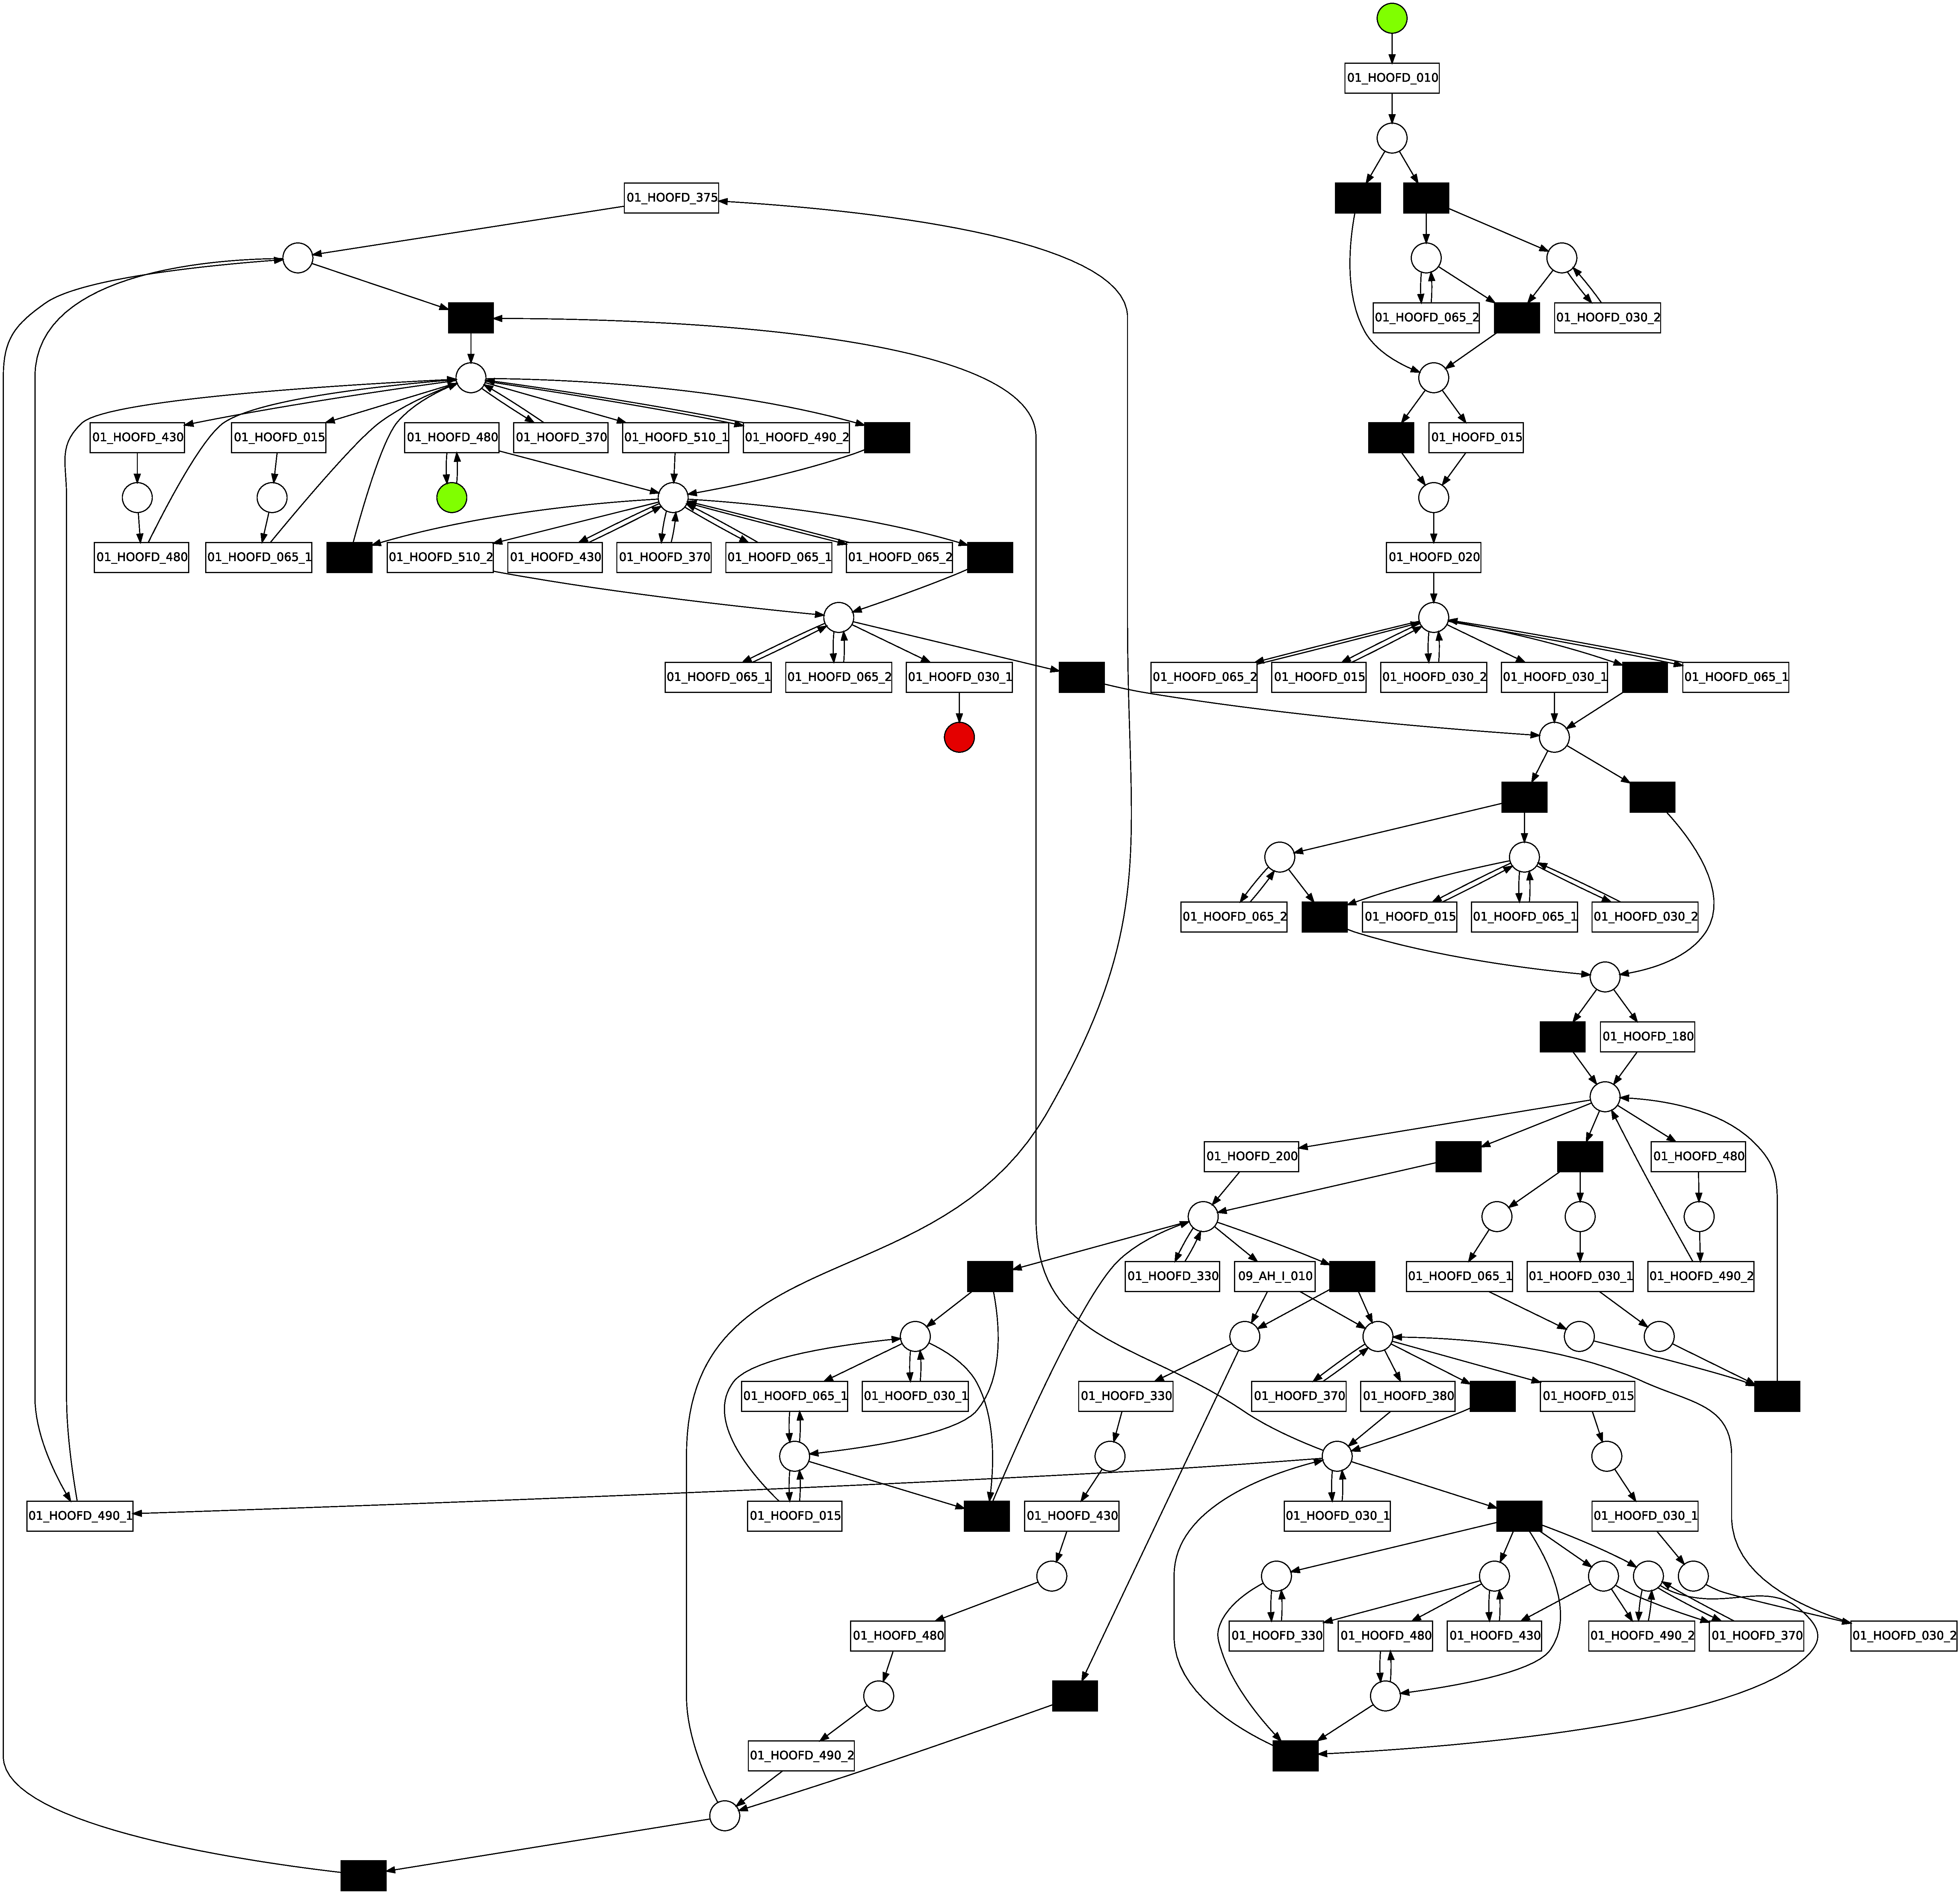
\includegraphics[width=1.0\textwidth, height=0.9\textheight]{figures/evaluation/PN-result-D4-3-M3-fahland-new.pdf}
		\caption{repaired model with Fahland}
		\label{fig:rl_fahland}
	\end{subfigure}%
	\begin{subfigure}[b]{0.43\textwidth}
		\centering
		
\includegraphics[width=.9\textwidth, height=0.9\textheight]{figures/evaluation/PN-result-D4-3-M3-dfg-05-1-05.pdf}
		\caption{repaired model with Dfg-repair}
		\label{fig:rl_dfg}
	\end{subfigure}
	\caption{Repaired model for $M_3$ based on event log D3.1 with positive instances for Fahland's repair techniques  while event log D3.3 with both positive and negative instances for Dfg-repair. The weight setting for Dfg-repair is 0.5 for the existing model, 1 for positive and 0.5 for negative instances. Default setting is chosen for Fahland's method.}
\end{figure}


\begin{table}[ht]
	\centering
	\caption{Test Result on BPI15-M1 data}
	\label{tab:rl-result}
	\resizebox{\textwidth}{!}{
		\begin{tabular}{lll|llllllll|}
			\hline
			\multirow{2}{*}{\thead{event \\ log}} & \multirow{2}{*}{\thead{reference \\ model} }                &    \multirow{2}{*}{\thead{method}}       & \multicolumn{8}{l|}{ \thead{confusion matrix metrics}}                                \\
			\cline{4-11}
			&  &     &
			\thead{TP}  & \thead{FP} & \thead{TN}  & \thead{FN}  & \thead{recall} & \thead{precision} & \thead{accuracy} & \thead{F1}             \\
			\hline
			D3.1      & -              & IM & 137 & 48 & 118 & 289 & 0.32   & 0.74      & 0.43     & 0.45                \\
			D3.1      & M1              & Fahland   & 343   & 136  &10     &6     &0.983        & 0.716           &   0.713       & 0.829         \\
			
			D3.3      & M1              & Dfg-repair:1-1-1       &  124   &  52  &  94   &    225 &   0.355     &     0.705      & 0.44         & 0.472            \\
			D3.3      & M1              & Dfg-repair:0.5-1-0.5       &  155   &  66  &  80   &    194 &   0.444     &     0.701     & 0.474         & 0.544            \\
			\hline
			D3.1      & M2              & Fahland   & 317    & 133   &   13  & 32    &  0.908      &    0.704       & 0.667         &  0.793   \\
			
			D3.3      & M2              & Dfg-repair:1-1-1       & 124    &   52 &   94  & 225    &  0.355      &   0.705        &  0.44         &  0.472      \\
			
			D3.3      & M2              & Dfg-repair:0.5-1-0.5       & 155    &   66 &   80  & 194    &  0.444      &   0.701        &  0.475         &  0.544      \\
			\hline
			D3.1      & M3              & Fahland   & 349    & 145   &  1   &  0   &  1.0      &   0.706        &   0.707       &  0.828    \\
			
			D3.3      & M3              & Dfg-repair:1-1-1       &  0   &   0 &  146   &  349   &  0      &   NaN        &  0.295       &   0      \\
			D3.3      & M3              & Dfg-repair:0.5-1-0.5       &  132   &   63 &  83   &  217   &  0.378      &   0.677        &  0.434        &   0.485      \\
			\hline
			
			D3.1      & M4              & Fahland   &  349   & 144   &  2   &  0   & 1.0       &   0.708        &   0.709       &  0.829         \\
			
			D3.3      & M4              & Dfg-repair:1-1-1       &  0   &  0  &   146  &  349   &  0     &      NaN     & 0.294        & 0   \\
			D3.3      & M4              & Dfg-repair:0.5-1-0.5       &  125   &  59  &   87  &  224   &  0.358     &      0.679     & 0.428        & 0.469   \\
			\hline
			D4.1      & -              & IM &  131   &  21  & 128    &  215   &    0.379    & 0.862           &   0.523       &    0.526     \\
			D4.1      & M1              & Fahland   &  325   &  133  &  16   & 21    &   0.939     &  0.710         &  0.689       & 0.808                \\
			
			D4.3      & M1              & Dfg-repair:1-1-1       &  139   & 36   & 113    &   207  &   0.402     &   0.794        &   0.509       &   0.534                   \\
			D4.3      & M1              & Dfg-repair:0.5-1-0.5       &  172   & 48   & 101    &   174  &   0.497     &   0.782       &   0.552       &   0.608                   \\
			\hline
			D4.1      & M2              & Fahland   & 325    &  130  & 19    &  21   & 0.939       &    0.714       &  0.695        &  0.811                \\
			
			D4.3      & M2              & Dfg-repair:1-1-1     &  139   & 36   & 113    &   207  &   0.402     &   0.794        &   0.509       &   0.534              \\
			D4.3      & M2              & Dfg-repair:0.5-1-0.5     &  172   & 48   & 101    &   174  &   0.497     &   0.782        &   0.552       &   0.608              \\
			\hline
			D4.1      & M3              & Fahland   & 87    &  29  & 120    &  259   & 0.251       &    0.75       &  0.418        &  0.377                    \\
			D4.3      & M3              & Dfg-repair:1-1-1       &  0   &  0  & 346    &  149   &  0      &   NaN        &   0.303       &  0       \\ 
			D4.3      & M3              & Dfg-repair:0.5-1-0.5       &  182   &  49  & 164    &  100   &  0.526      &   0.788        &   0.70       &  0.631      \\ 
			
			\hline
			D4.1      & M4              & Fahland   & 63    &  20  & 129    &  283   & 0.182       &    0.759       &  0.388        &  0.294                 \\
			
			D4.3      & M4              & Dfg-repair:1-1-1       &   0  & 0   &  346   & 149    &   0     &    NaN       &     0.303     &  0      \\  
			D4.3      & M4              & Dfg-repair:0.5-1-0.5       &   172  & 48   &  101   & 174    &   0.497     &    0.782       &     0.552     &  0.608      \\      
			\hline              
	\end{tabular}}
\end{table}
% add some analysis on them..

As the results shown in Table \ref{tab:rl-result}, Fahland's repair techniques from \cite{fahland2015model} tend to have high recall but low values for true and false negative. The possible reasons are that (1) it repairs the reference model with the positive instances, which addresses the fitness of positive traces. (2) it repairs the model by adding subprocesses and introduces more behavior into the model, which also allows for the negative instances. Inductive Miner rediscovers a new model from the given positive instances, while the reference models are simply ignored. As a result, the generated model in Figure \ref{fig:rl_IM} has changed a lot compared to the original model M3 as shown in the Figure \ref{fig:rl_ref}.  

Dfg-repair techniques uses control parameters to balance the forces from the existing model, positive and negative instances. Therefore, with different setting, Dfg-repair techniques repair the model in different ways. To address this phenomenon, besides the default setting with value 1 for all parameters, another setting with 0.5 for the existing model, 1 for the positive instances, 0.5 for the negative instances is used to conduct experiments. As shown in the Table \ref{tab:rl-result}, with different settings, the repaired models change. Compared to the default setting, the setting with values 0.5, 1 and 0.5 results in models with higher recall, accuracy, and F1 score. The reasons behind might be that the force from negative instances affects model a lot, with the weight 1.0. It possibly blocks the behavior which contributes to positive performances.  With lower value on it, the forces from the existing model, positive and negative are balanced better and the quality of the repaired model is improved. As an example, the experiments on D3.3 and M3, or D.3. and M4, which shows the quality changes due to different setting.

Except for the weight for negative instances, the weight for the existing model also affects the quality of repaired model. The influence of the weights on the repaired model is analyzed later in the section. 


Due to the different settings in our method, forces from the reference model, positive, and negative event logs are balanced differently during repair, which results in different process models. To investigate the effect of those setting on the repaired model, we repeat our experiments on the following setting. 

Each of three control parameters for the existing model, positive and negative instances changes value from 0.0 to 1.0 with step 0.1. With this setting, directly-follows relation is generated. Afterward, the default setting of Inductive Miner Infrequent with noise threshold 20 is used to mine Petri nets from the generated directly-follows graph. In total, thousand experiments are conducted to investigate Dfg-repair method. Based on those results, we draw plots to show the tendency of evaluation results on the parameters for the existing model, positive and negative event logs. 

\begin{figure}[htb]
	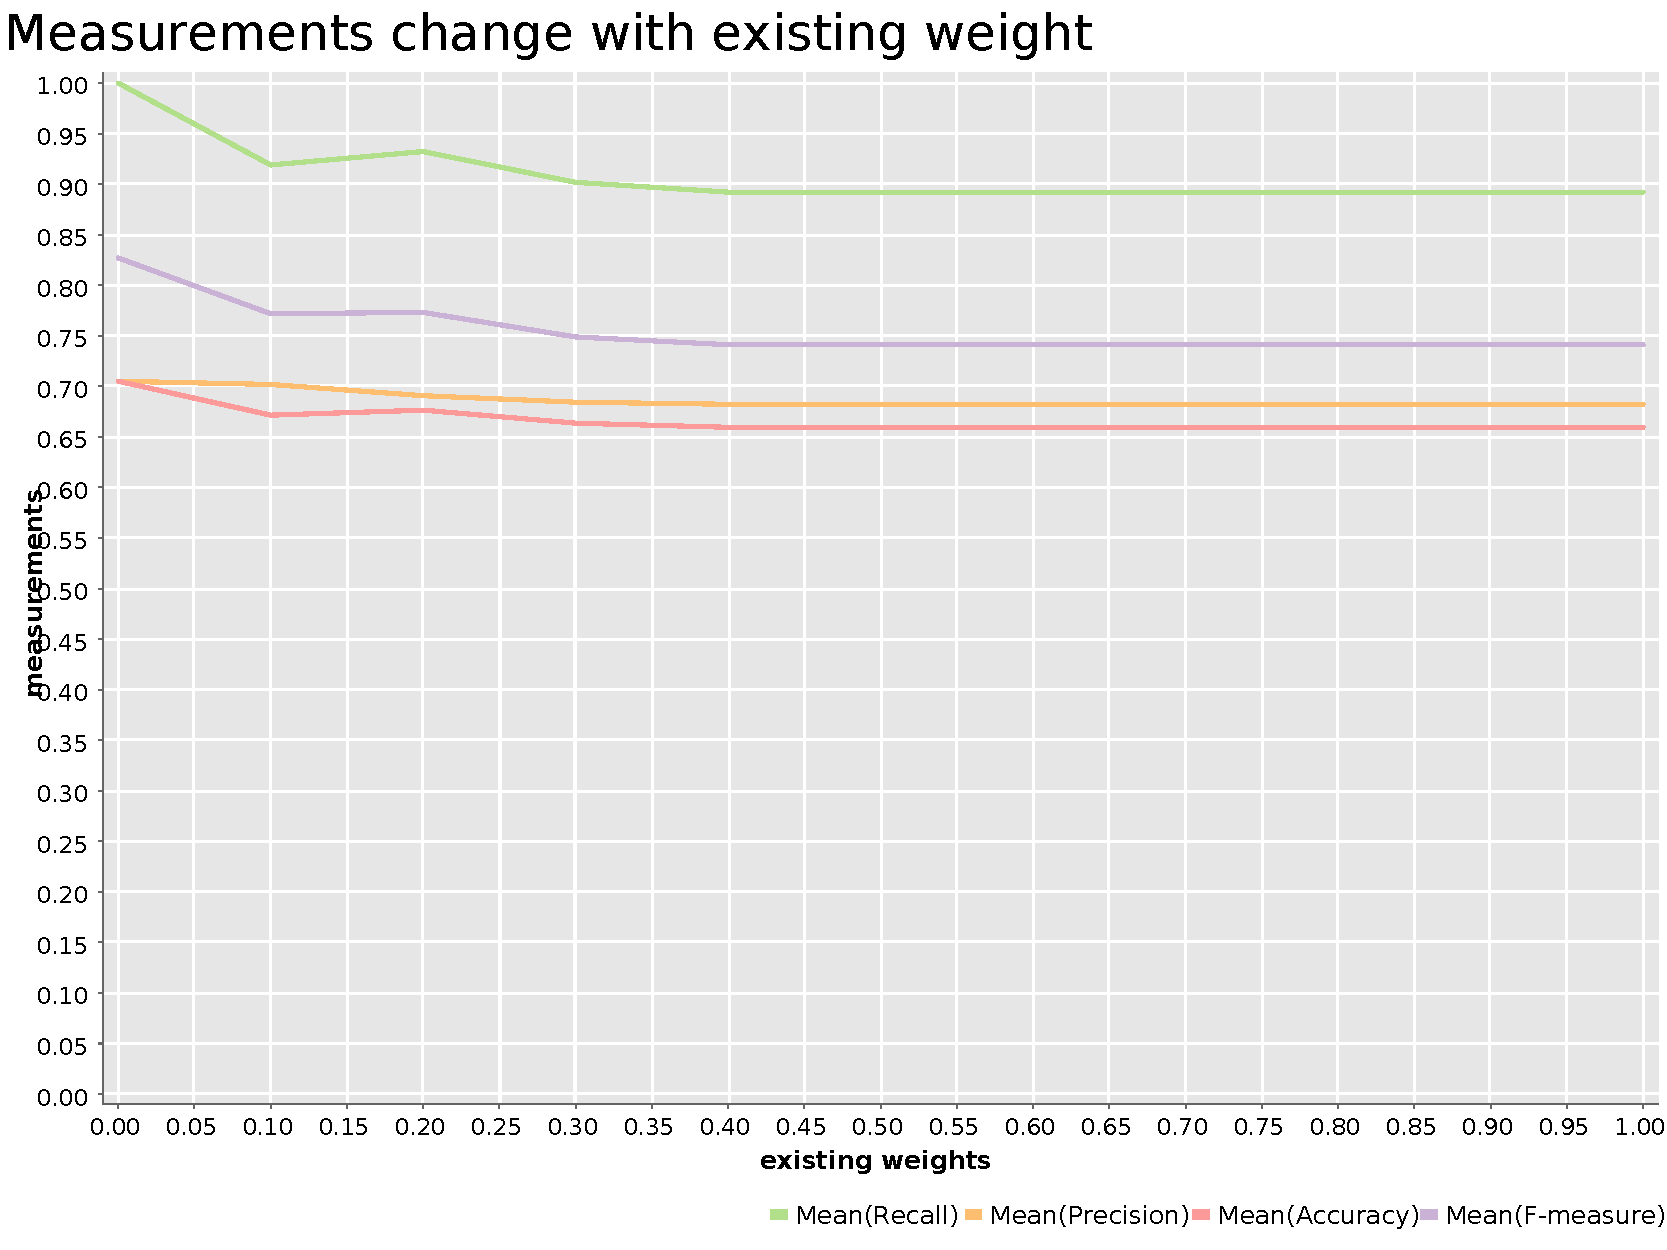
\includegraphics[width=\linewidth]{figures/evaluation/M3-D43-ext-weight-plot.pdf}
	\caption{result with control parameter for existing model on event log D3.3 and model M3}
	\label{fig:ext-weight}
\end{figure} 
From the Figure \ref{fig:ext-weight}, with the parameter for the existing model going up, recall goes up while accuracy and precision goes down. The reason behind it is possibly ????.


\begin{figure}[htb]
	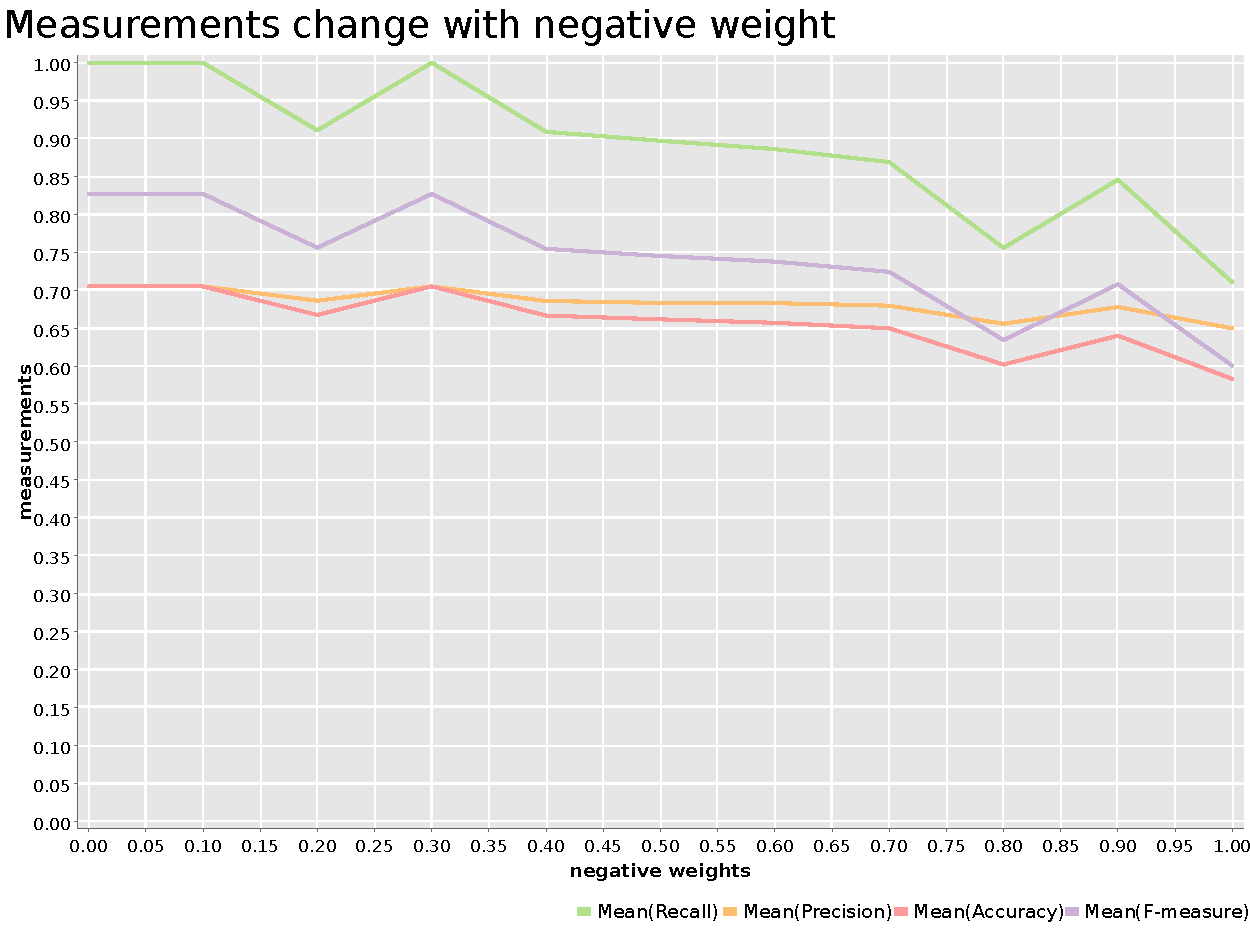
\includegraphics[width=\linewidth]{figures/evaluation/M3-D43-neg-weight-plot.pdf}
	\caption{result with control parameter for negative instance on event log D3.3 and model M3}
	\label{fig:neg-weight}
\end{figure}
Figure \ref{fig:neg-weight} shows that if the parameter for negative event log increases, precision and accuracy go up. By addressing negative force, our techniques tend to block behavior which leads to low performance output. However, if the negative force is over the force from positive event log and the existing model, certain behavior which contributes to positive performance will also be deleted from the models. In contrast, this creates a model with less recall. 


\begin{figure}[htb]
	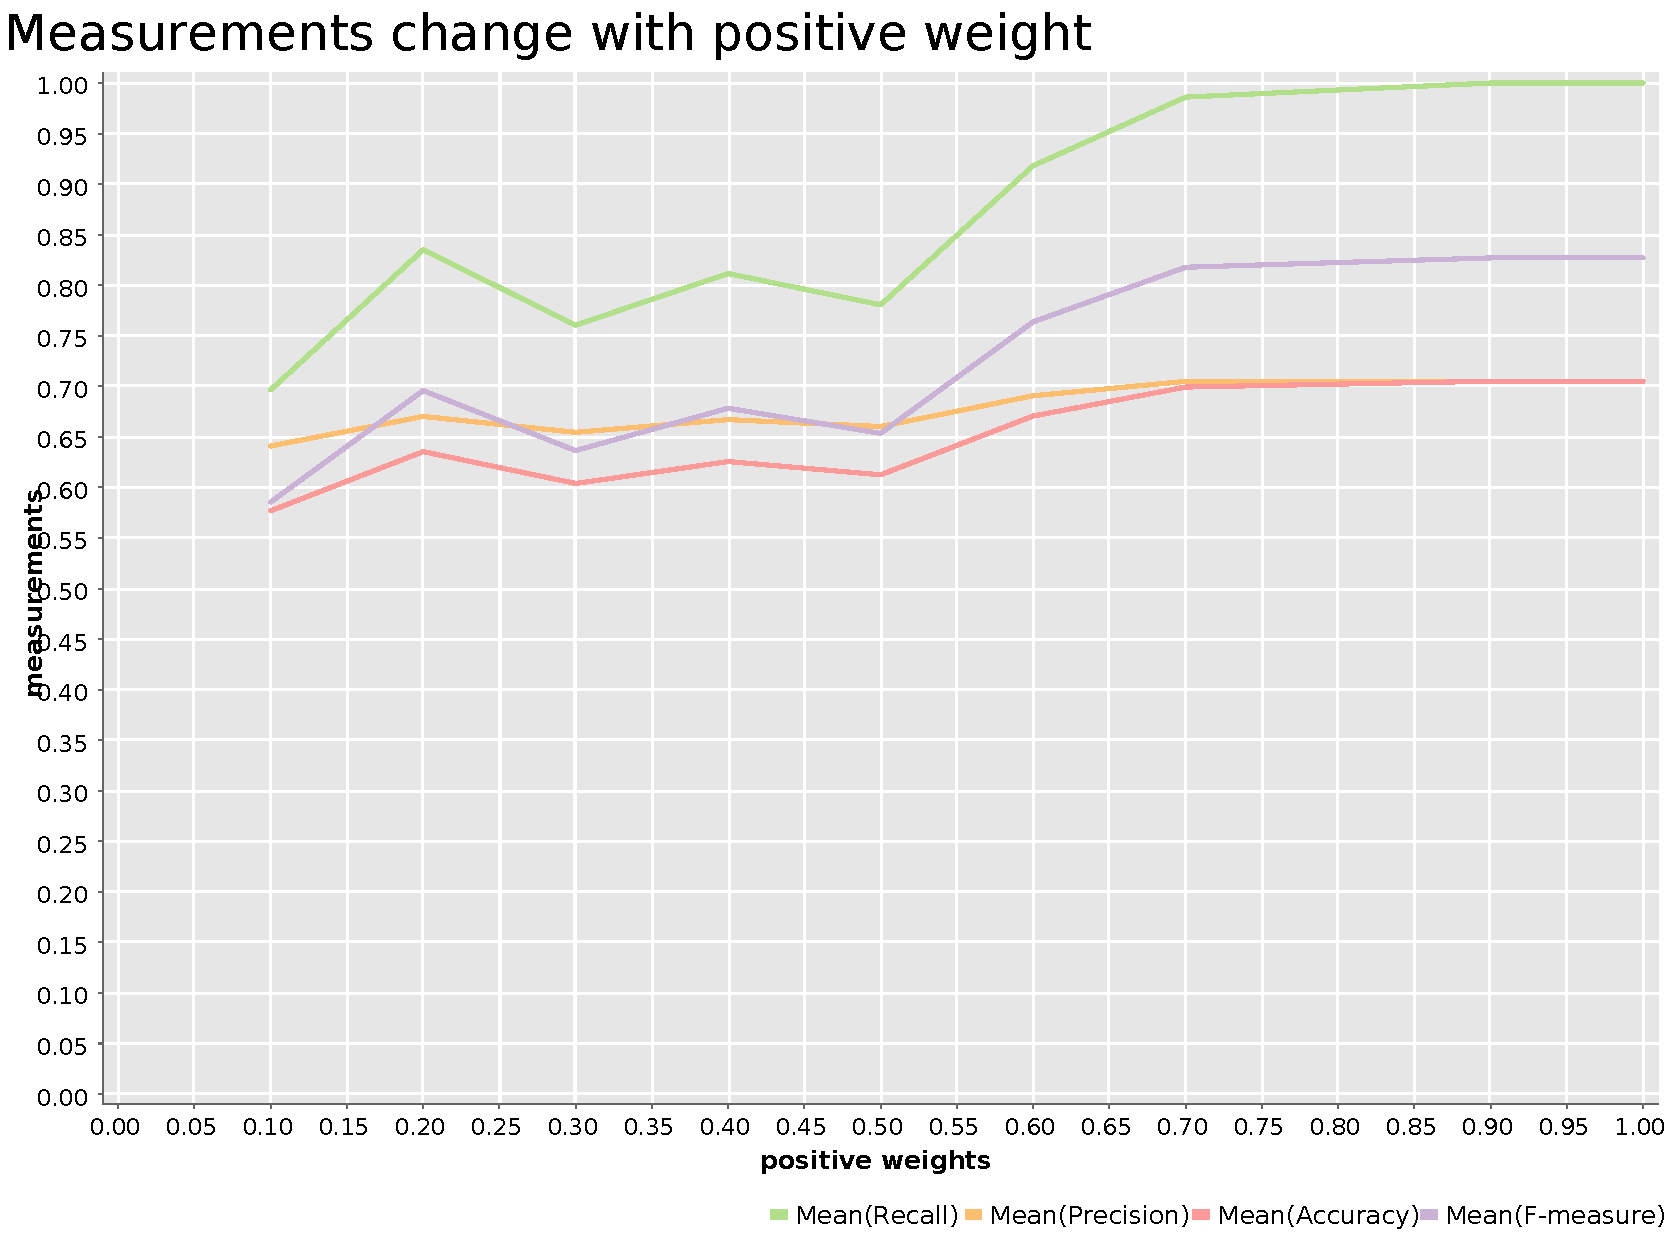
\includegraphics[width=\linewidth]{figures/evaluation/M3-D43-pos-weight-plot.pdf}
	\caption{result with control parameter for positive instance on event log D3.3 and model M3}
	\label{fig:pos-weight}
\end{figure}
Figure \ref{fig:pos-weight} displays the tendency with the parameter for positive event log. When the positive parameter rises, the recall increases. Precision and accuracy also increases but with ???.